\section{Kiến trúc tổng thể của hệ thống}
Hệ thống chatbot phát hiện lừa đảo điện thoại cho người cao tuổi được thiết kế theo mô hình nhiều tầng (Multi-layer Architecture), bao gồm năm thành phần chính: thiết bị người dùng, tầng trung chuyển bảo mật, tầng xử lý trung tâm, tầng tri thức cục bộ và tầng trí tuệ nhân tạo. Kiến trúc này được xây dựng theo hướng Retrieval-Augmented Generation (RAG), cho phép kết hợp tri thức chuyên biệt về các kịch bản lừa đảo với khả năng suy luận ngôn ngữ tự nhiên của mô hình ngôn ngữ lớn.

Ở tầng đầu tiên, người dùng tương tác với hệ thống thông qua giao diện Web trên máy tính hoặc thiết bị di động. Đây là điểm tiếp xúc trực tiếp giữa người cao tuổi và chatbot. Người dùng có thể nhập nội dung cuộc gọi hoặc đoạn hội thoại cần kiểm tra để yêu cầu hệ thống đánh giá mức độ rủi ro.

Các yêu cầu từ giao diện được gửi qua Internet đến FastAPI Backend. Trong giai đoạn phát triển và trình diễn, hệ thống được triển khai trên nền tảng Render -- một dịch vụ đám mây cho phép chạy ứng dụng web nhanh chóng mà không cần mở trực tiếp cổng mạng ra Internet. Tuy nhiên, gói miễn phí của Render có một hạn chế: nếu không có ai dùng trong vòng 15 phút, hệ thống sẽ tự động tắt để tiết kiệm tài nguyên. Khi có yêu cầu mới, Render phải khởi động lại ứng dụng từ đầu, mất khoảng 30 đến 50 giây trước khi có thể trả lời. Vì vậy, môi trường này chỉ phù hợp để trình diễn và thử nghiệm, không dùng để vận hành thực tế.

Sau khi nhận được yêu cầu, FastAPI Backend đóng vai trò là trung tâm điều phối toàn bộ quá trình xử lý. Backend tiếp nhận nội dung hội thoại, thực hiện tiền xử lý ngôn ngữ, truy xuất cơ sở tri thức cục bộ và xây dựng ngữ cảnh cho mô hình AI. Dữ liệu tri thức được lưu trữ dưới dạng các tệp JSON trong thư mục Data\_Kich\_Ban, bao gồm nhiều loại hình lừa đảo phổ biến như giả danh cơ quan nhà nước, lừa đảo đầu tư tài chính, lừa đảo tiền ảo, lừa đảo định danh điện tử hoặc các hình thức lừa đảo mới được cập nhật theo thời gian.

Thông qua cơ chế Retrieval-Augmented Generation, hệ thống sẽ truy xuất các kịch bản liên quan từ kho tri thức, sau đó kết hợp với System Prompt và nội dung cuộc hội thoại hiện tại để tạo thành một Prompt hoàn chỉnh. Prompt này được gửi đến Groq Cloud API sử dụng mô hình Llama-3.1-8B-Instant nhằm thực hiện quá trình suy luận. Trong trường hợp Groq gặp lỗi tạm thời, cơ chế thử lại được kích hoạt với tối đa hai lần thử và thời gian chờ tăng dần (exponential backoff). Nếu tất cả các lần thử đều thất bại, OpenRouter API được sử dụng làm kênh dự phòng (fallback).

Tầng trí tuệ nhân tạo thực hiện các tác vụ phân tích ngôn ngữ tự nhiên và đánh giá rủi ro. Dựa trên ngữ cảnh được cung cấp, mô hình xác định các dấu hiệu lừa đảo, đánh giá mức độ nguy hiểm và tạo phản hồi dưới dạng ngôn ngữ tự nhiên. Kết quả sau đó được đưa qua tầng kiểm soát HallucinationGuard nhằm phát hiện và loại bỏ các thông tin bịa đặt trước khi gửi lại cho người dùng.

Việc tách biệt rõ ràng các tầng chức năng giúp hệ thống dễ dàng mở rộng trong tương lai, đồng thời tăng khả năng bảo trì, cập nhật cơ sở tri thức và thay thế mô hình AI mà không ảnh hưởng đến các thành phần còn lại.

\begin{figure}
    \centering
    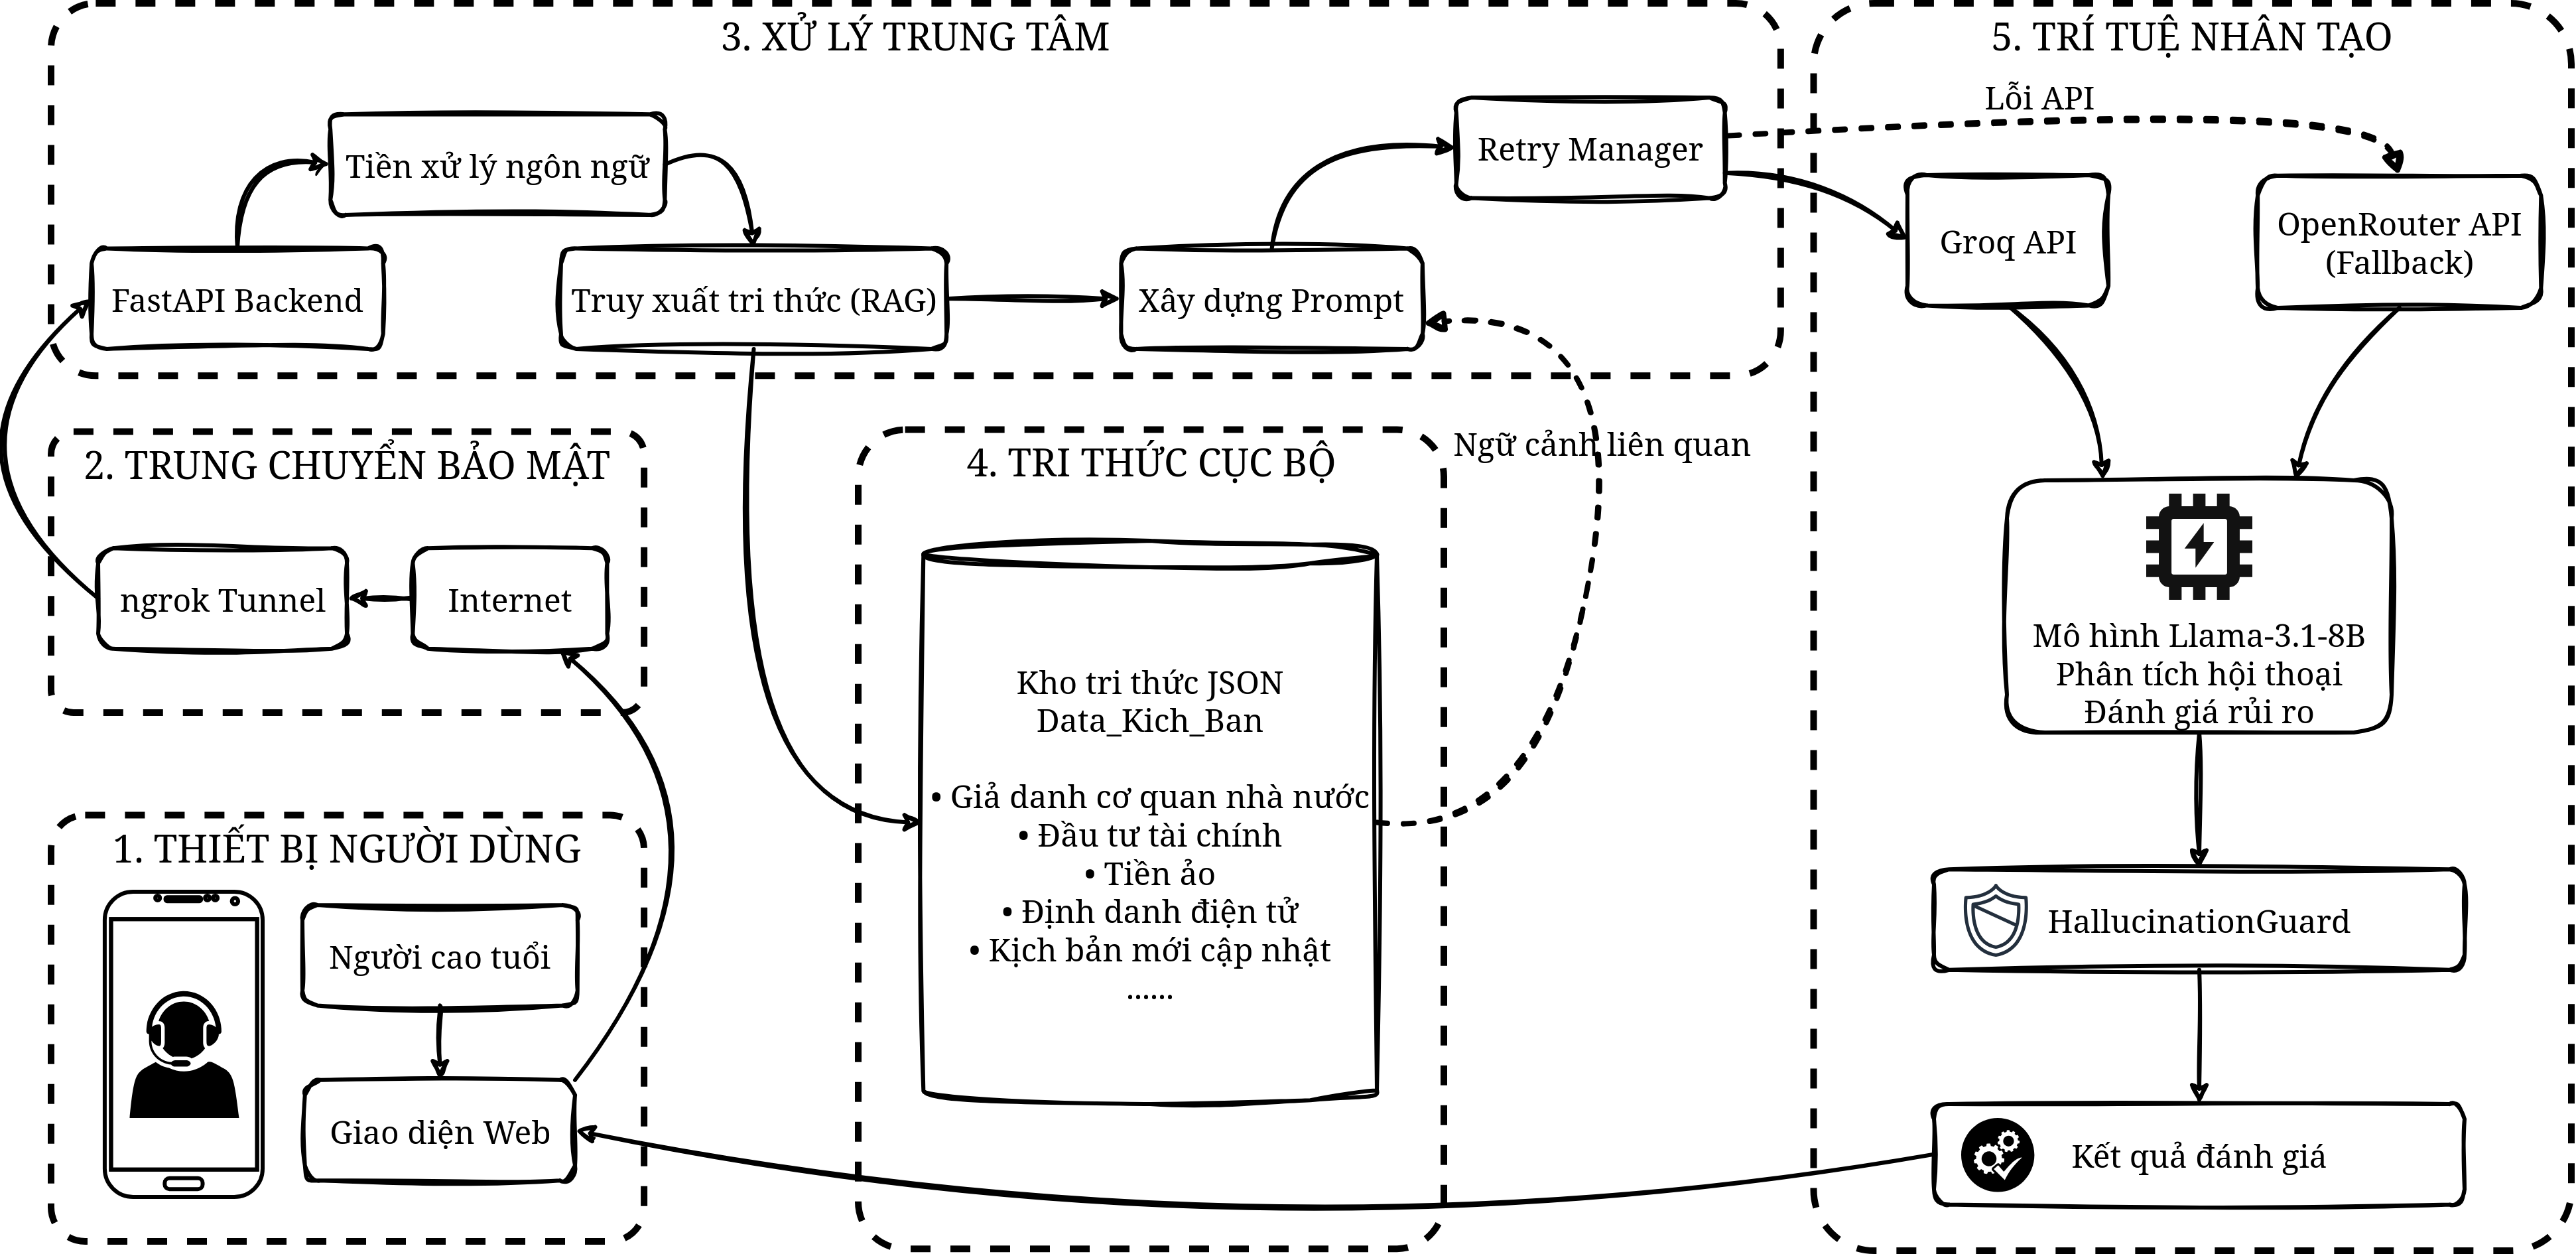
\includegraphics[width=1\linewidth]{kien-truc.png}
    \caption{Kiến trúc hệ thống đề xuất}
    \label{fig:kientruc}
\end{figure}

\section{Luồng hoạt động của hệ thống}
Quá trình xử lý một yêu cầu từ người dùng gồm 12 bước như sau.
\begin{itemize}
    \item Bước 1: Người dùng nhập nội dung cuộc gọi trên giao diện Web, dữ liệu được gửi đến hệ thống dưới dạng JSON.

    \item Bước 2: Render (môi trường demo) tiếp nhận yêu cầu và chuyển tiếp đến FastAPI Backend.

    \item Bước 3: Backend phát hiện và điều chỉnh xưng hô dựa vào đầu vào, sử dụng bảng ánh xạ 33 đại từ nhân xưng (XUNG\_HO\_MAP) và bảy mẫu phát hiện. Ví dụ, nếu người dùng tự xưng "cháu" và gọi hệ thống là "cô", phản hồi dùng cặp "cô/cháu". Nếu người dùng nói "Con ơi", hệ thống nhận ra người lớn tuổi và dùng "con/..." (reverse lookup).

    \item Bước 4: DialectNormalizer chuẩn hóa phương ngữ qua từ điển hơn 110 mục (DIALECT\_MAP), ánh xạ từ địa phương miền Trung và miền Nam sang phổ thông (ví dụ: "mô" $\rightarrow$ "đâu", "răng" $\rightarrow$ "sao", "hổng" $\rightarrow$ "không"). Từ viết hoa ở giữa câu được giữ nguyên để tránh làm thay đổi tên riêng ("Chi" không thành "gì"). Từ viết hoa ở đầu câu vẫn được chuẩn hóa nhưng giữ nguyên chữ hoa đầu.

    \item Bước 5: Backend xác định vùng miền (Bắc, Trung, Nam) dựa trên dấu hiệu từ vựng, dùng ranh giới từ để tránh khớp nhầm (ví dụ "hông" trong "không"). Thông tin vùng miền và dạng chuẩn hóa đầu tiên của câu hỏi được lưu làm "neo" cho các truy vấn RAG ở lượt sau, tránh trôi ngữ cảnh.

    \item Bước 6: Backend quét thư mục Data\_Kich\_Ban, đọc các tệp JSON tri thức. Mỗi khối dữ liệu được tính điểm dựa trên số từ khóa xuất hiện trong câu hỏi. Từ khóa nhiều từ (ví dụ: "chuyển khoản", "mã OTP") được kiểm tra dưới dạng chuỗi con thay vì so khớp rời rạc từng từ. Nếu có từ hai từ khóa trở lên khớp, khối được đưa vào ngữ cảnh; nếu không đủ điểm, khối bị bỏ qua.

    \item Bước 7: Ngữ cảnh RAG được ghép với System Prompt và nội dung hội thoại hiện tại. Hệ thống áp dụng hai chế độ:
    \begin{itemize}
        \item Lượt 1: Dùng ngữ cảnh RAG, System Prompt đầy đủ với cấu trúc ba dòng (chào + nhận dạng / giải thích / lời khuyên).
        \item Lượt 2+: Chuyển sang hội thoại tự do, không dùng RAG, không lặp lại lời chào hay cấu trúc cứng nhắc.
    \end{itemize}

    \item Bước 8: Gọi API Groq với cơ chế thử lại (tối đa hai lần, chờ 1s và 2s). Nếu thất bại, chuyển sang OpenRouter. Nếu cả hai đều lỗi, trả về mã 503 kèm thông báo hệ thống tạm thời không khả dụng.

    \item Bước 9: HallucinationGuard kiểm tra phản hồi: trích xuất các khẳng định, tính điểm neo (grounding score) dựa trên mức độ khớp với ngữ cảnh RAG và nội dung hội thoại, đồng thời phát hiện các mẫu không an toàn. Nếu điểm dưới ngưỡng, phản hồi được thay bằng thông báo thận trọng hơn.

    \item Bước 10: Hệ thống định dạng lại phản hồi thành ba dòng: dòng 1 -- lời chào và nhận dạng rủi ro, dòng 2 -- giải thích, dòng 3 -- lời khuyên. Ở các lượt sau, nếu người dùng gửi "cảm ơn" hoặc "hiểu rồi" mà không kèm câu hỏi, hệ thống phát hiện ý định kết thúc và trả lời chào tạm biệt ngắn gọn.

    \item Bước 11: Backend đóng gói kết quả thành JSON gồm văn bản phản hồi, xưng hô đã phát hiện, vùng miền, số lượt hội thoại và gửi về giao diện Web.

    \item Bước 12: Giao diện hiển thị phản hồi dưới dạng văn bản tự nhiên. Dù trình bày tự do, phản hồi vẫn tuân theo cấu trúc logic: nhận định rủi ro, giải thích lý do dựa trên dấu hiệu phát hiện được, và lời khuyên hành động. Cấu trúc này được đảm bảo qua System Prompt và hậu xử lý.
\end{itemize}

Quy trình xử lý dữ liệu qua các bước được minh họa trong Hình~\ref{fig:luong_xu_ly}.

\begin{figure}[H]
    \centering
    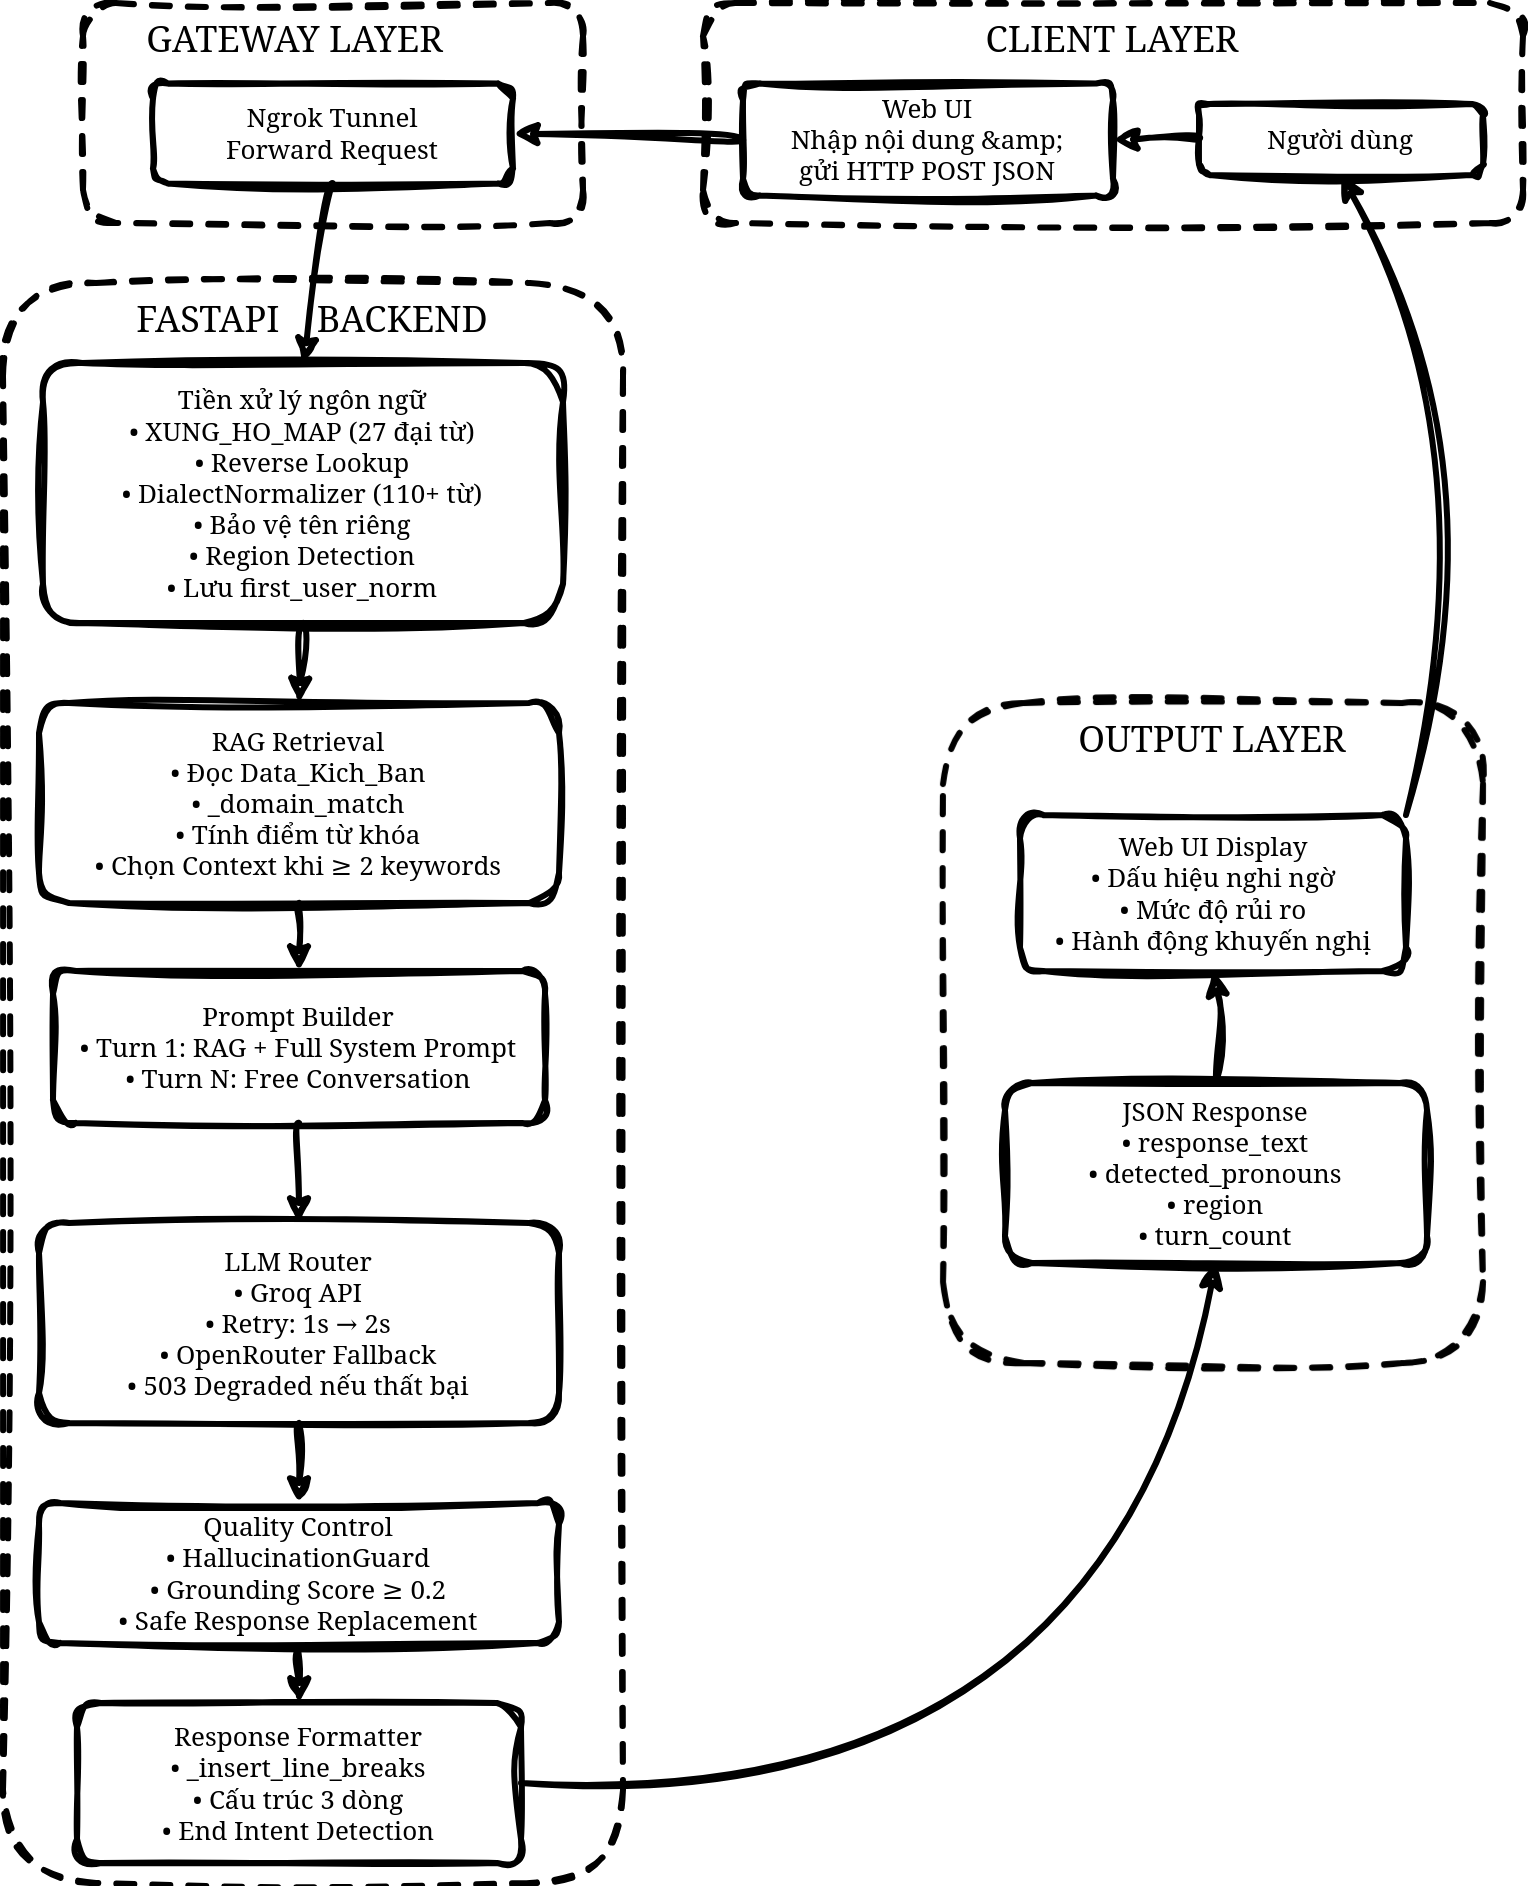
\includegraphics[width=1\linewidth]{luong-xu-li.png}
    \caption{Luồng xử lý của dữ liệu}
    \label{fig:luong_xu_ly}
\end{figure}
